\documentclass[12pt]{article}

% ============================================================
% IDIOMA Y CODIFICACIÓN
% ============================================================
\usepackage[spanish]{babel}
\usepackage[utf8]{inputenc}
\usepackage[T1]{fontenc}

% ============================================================
% MÁRGENES Y GEOMETRÍA
% ============================================================
\usepackage[a4paper, margin=2.5cm]{geometry}

% ============================================================
% ESPACIADO MEJORADO
% ============================================================
\usepackage{setspace}
\setstretch{1.15}

\setlength{\parskip}{0.5em}
\setlength{\parindent}{0pt}

% Margen extra de elasticidad para los párrafos con nombres de variables
% y de archivos en \texttt, que no admiten corte de línea
\setlength{\emergencystretch}{1.5em}

% ============================================================
% TIPOGRAFÍA
% ============================================================
\usepackage{lmodern}

% ============================================================
% COMILLAS TIPOGRÁFICAS (compatibles con babel/español)
% ============================================================
\usepackage{csquotes}

% ============================================================
% FORMATO DE TÍTULOS
% ============================================================
\usepackage{titlesec}

\titleformat{\section}
  {\Large\bfseries}
  {\thesection.}
  {0.5em}
  {}

\titlespacing*{\section}{0pt}{1.5em}{0.8em}

% ============================================================
% MATEMÁTICAS
% ============================================================
\usepackage{amsmath, amssymb, amsfonts}

% ============================================================
% GRÁFICOS
% ============================================================
\usepackage{graphicx}
\usepackage{caption}

% ============================================================
% TABLAS
% ============================================================
\usepackage{booktabs}
\usepackage{array}
\usepackage{multirow}
\usepackage{longtable}

% ============================================================
% CÓDIGO / PYTHON
% ============================================================
\usepackage{listings}
\usepackage{xcolor}

\definecolor{codebg}{RGB}{248, 248, 248}
\definecolor{codeframe}{RGB}{200, 200, 200}
\definecolor{codecomment}{RGB}{106, 153, 85}
\definecolor{codekeyword}{RGB}{86, 156, 214}
\definecolor{codestring}{RGB}{206, 145, 120}
\definecolor{codenumber}{RGB}{181, 206, 168}

\lstdefinestyle{estilo_base}{
    backgroundcolor=\color{codebg},
    frame=single,
    rulecolor=\color{codeframe},
    basicstyle=\ttfamily\small,
    commentstyle=\color{codecomment}\itshape,
    keywordstyle=\color{codekeyword}\bfseries,
    stringstyle=\color{codestring},
    numberstyle=\tiny\color{codenumber},
    numbers=left,
    numbersep=8pt,
    breaklines=true,
    breakatwhitespace=true,
    tabsize=4,
    showstringspaces=false,
    captionpos=b,
    literate=
        {á}{{\'a}}1 {é}{{\'e}}1 {í}{{\'i}}1 {ó}{{\'o}}1 {ú}{{\'u}}1
        {Á}{{\'A}}1 {É}{{\'E}}1 {Í}{{\'I}}1 {Ó}{{\'O}}1 {Ú}{{\'U}}1
        {ñ}{{\~n}}1 {Ñ}{{\~N}}1 {ü}{{\"u}}1 {¿}{{?`}}1 {¡}{{!`}}1
        {°}{{\textdegree}}1,
}

% Estilo para código Python
\lstdefinestyle{python}{
    style=estilo_base,
    language=Python,
}
\renewcommand{\lstlistingname}{Código}

\newcommand{\codigo}[1]{\texttt{\small #1}}

% ============================================================
% COMANDO PARA LA SALIDA POR CONSOLA
% ============================================================
\lstdefinestyle{salida}{
    style=estilo_base,
    numbers=none,
    basicstyle=\ttfamily\scriptsize,
    keywordstyle=\color{black},
    commentstyle=\color{black},
    stringstyle=\color{black},
    breaklines=false,
}

% ============================================================
% LISTAS
% ============================================================
\usepackage{enumitem}

% ============================================================
% ENLACES
% ============================================================
\usepackage{hyperref}
\hypersetup{
    colorlinks  = true,
    linkcolor   = black,
    urlcolor    = blue!60!black,
    citecolor   = black,
    pdftitle    = {Examen Final Integrador - Programación II},
    pdfauthor   = {Facundo Luna},
}

% ============================================================
% ENCABEZADO Y PIE DE PÁGINA
% ============================================================
\usepackage{fancyhdr}
\pagestyle{fancy}
\fancyhf{}
\renewcommand{\headrulewidth}{0.4pt}
\renewcommand{\footrulewidth}{0.4pt}
\fancyhead[L]{\small Programación II}
\fancyhead[R]{\small Examen Final Integrador}
\fancyfoot[L]{\small Facundo Luna}
\fancyfoot[R]{\small \thepage}

% ============================================================
% DATOS DEL TRABAJO
% ============================================================

\newcommand{\universidad}{Universidad Católica de Salta}
\newcommand{\carrera}{Licenciatura en Ciencia de Datos}
\newcommand{\materia}{Programación II}
\newcommand{\trabajo}{Examen Final Integrador}
\newcommand{\profesor}{Ing. Mario Martínez}
\newcommand{\alumno}{Facundo Luna}
\newcommand{\aniolectivo}{2026}
\newcommand{\fecha}{\today}

\newcommand{\logoincluido}{%
    
\includegraphics[width=3.5cm]{../../../assets/ucasal-logo.png}\\[0.5cm]%
}
\newcommand{\logoomitido}{\vspace{1cm}}

\newcommand{\logoportada}{\logoincluido}

% ============================================================
% COMANDO VOLVER AL ÍNDICE
% ============================================================
\newcommand{\volverindice}{%
    \vspace{1em}%
    \begin{flushright}%
        \hyperlink{indice}{\small $\uparrow$ Volver al índice}%
    \end{flushright}%
}

% ============================================================
% COMANDO PARA EL ENUNCIADO
% ============================================================
\newcommand{\enunciado}[1]{%
    \begin{quote}
        \itshape #1
    \end{quote}
}

% ============================================================

\begin{document}

% ======================== PORTADA ===========================

\begin{titlepage}
    \centering

    \logoportada

    \rule{\linewidth}{1.5pt}\\[0.4cm]

    {\large\scshape \universidad}\\[0.2cm]
    {\large \carrera}\\[0.1cm]

    \rule{\linewidth}{0.5pt}\\[1.5cm]

    {\Huge\bfseries \trabajo}\\[0.8cm]
    {\LARGE \materia}\\[1.2cm]

    {\large\itshape Sistema de control de gestión de sucursal}\\[2cm]

    \begin{tabular}{rl}
        \textbf{Alumno:}       & \alumno       \\[0.3cm]
        \textbf{Profesor:}     & \profesor     \\[0.3cm]
        \textbf{Año lectivo:}  & \aniolectivo  \\[0.3cm]
        \textbf{Fecha:}        & \fecha        \\
    \end{tabular}

    \vfill

    \rule{\linewidth}{1.5pt}

\end{titlepage}

% ======================== ÍNDICE ============================

\newpage
\tableofcontents
\hypertarget{indice}{}
\setcounter{tocdepth}{2}

% ======================== CUERPO ============================

\newpage

\phantomsection
\section*{Aclaraciones previas}
\addcontentsline{toc}{section}{Aclaraciones previas}

El presente trabajo corresponde al examen final integrador de Programación II. La consigna de la cátedra pide tomar como base el Ejercicio 14 del Trabajo Práctico N° 4 y mejorarlo incorporando más herramientas y complejidad, presentando tanto el enunciado del ejercicio como su programación en Python.

Siguiendo la recomendación de la cátedra, se conservó el tema del Ejercicio 14 (el análisis anual de ventas y merma de una sucursal de supermercado) y se lo extendió hasta convertirlo en un sistema de consulta completo. La elección del tema no responde únicamente a esa continuidad: quien suscribe trabaja actualmente en un supermercado, por lo que se trata de un dominio conocido de primera mano. Eso es lo que permitió que el criterio central del trabajo, la meta de merma propia de cada sector, esté tomado de cómo se controla efectivamente la mercadería en una sucursal (no es lo mismo lo que se puede descartar en limpieza que en verdulería) y no de valores elegidos al azar para completar el ejercicio. La sección \ref{sec:mejoras} detalla punto por punto qué se agregó respecto de aquella versión.

El proyecto está formado por los siguientes archivos:

\begin{itemize}[leftmargin=1.5em, itemsep=0.2em]
    \item \codigo{Examen\_Final.py}: el programa, con el apellido y nombre del alumno en la primera línea de comentario, según el formato exigido por la cátedra.
    \item \codigo{ventas.csv}: el archivo de ventas del Ejercicio 14, con 72 registros (12 meses por 6 sectores).
    \item \codigo{sectores.csv}: archivo nuevo, con la ficha de cada sector.
    \item \codigo{programacion2-examen-final-facundo-luna.pdf}: este documento.
\end{itemize}

El programa se ejecuta desde la carpeta donde están los dos archivos CSV, ya que los abre por su nombre y no por una ruta absoluta. Requiere las bibliotecas \codigo{numpy} y \codigo{matplotlib}.

\newpage

% ============================================================
\section{Enunciado del ejercicio}
% ============================================================

\subsection{Planteo del problema}

Una sucursal de supermercado factura todos los meses, pero una parte de la mercadería nunca llega a venderse: se vence, se rompe o se descarta por mal estado. Esa pérdida se denomina \textbf{merma} y, al igual que la facturación, se mide en dinero.

El criterio habitual para controlarla es fijar un límite único de merma para toda la sucursal, que es lo que hacía el Ejercicio 14 del TP 4 con su constante del 3\,\%. Ese criterio tiene un problema: no todos los sectores enfrentan el mismo riesgo. Un sector de almacén vende mercadería que no se echa a perder, mientras que una verdulería trabaja con productos que se descartan en pocos días. Un límite común deja pasar al almacén que está perdiendo más de lo que debería y castiga a la verdulería que, en realidad, está dentro de lo esperable para su rubro.

El ejercicio consiste entonces en desarrollar un sistema de control de gestión que evalúe a cada sector contra su propia meta.

\subsection{Datos de entrada}

El sistema debe leer dos archivos CSV.

El primero, \codigo{ventas.csv}, tiene una fila por cada mes y sector:

\begin{center}
\begin{tabular}{lll}
    \toprule
    \textbf{Columna} & \textbf{Tipo} & \textbf{Descripción} \\
    \midrule
    \codigo{mes}              & entero & número de mes, de 1 a 12 \\
    \codigo{sector}           & texto  & nombre del sector de la sucursal \\
    \codigo{unidades}         & entero & unidades vendidas en el mes \\
    \codigo{precio\_unitario} & real   & precio de venta por unidad \\
    \codigo{unidades\_merma}  & entero & unidades perdidas en el mes \\
    \bottomrule
\end{tabular}
\end{center}

El segundo, \codigo{sectores.csv}, tiene una fila por sector con su ficha:

\begin{center}
\begin{tabular}{lll}
    \toprule
    \textbf{Columna} & \textbf{Tipo} & \textbf{Descripción} \\
    \midrule
    \codigo{sector}       & texto & nombre del sector, que vincula con \codigo{ventas.csv} \\
    \codigo{responsable}  & texto & encargado a cargo del sector \\
    \codigo{meta\_merma}  & real  & porcentaje de merma admitido para ese sector \\
    \codigo{categoria}    & texto & perecedero o no perecedero \\
    \bottomrule
\end{tabular}
\end{center}

\newpage
\subsection{Procesamiento solicitado}

A partir de esos datos, el sistema debe:

\begin{enumerate}[leftmargin=1.5em, itemsep=0.3em]
    \item Calcular, para cada sector, la facturación anual, la merma anual en dinero y el porcentaje que la merma representa sobre lo facturado:
    \[
        \text{facturación} = \text{unidades} \times \text{precio unitario}
        \qquad
        \text{merma} = \text{unidades de merma} \times \text{precio unitario}
    \]
    \[
        \%\ \text{merma} = \frac{\text{merma}}{\text{facturación}} \times 100
    \]

    \item Comparar ese porcentaje contra la meta propia del sector y asignarle un estado:
    \begin{itemize}[leftmargin=1.5em, itemsep=0.1em]
        \item \textbf{OK}: la merma real no supera la meta.
        \item \textbf{ATENCIÓN}: la supera, pero sin llegar a la meta multiplicada por una tolerancia del 20\,\%.
        \item \textbf{ALERTA}: supera ese margen de tolerancia.
        \item \textbf{SIN META}: el sector aparece en el archivo de ventas pero no tiene ficha cargada en el de sectores, de modo que no hay meta contra la cual compararlo. Sus ventas se informan igual.
    \end{itemize}

    \item Informar la evolución mes a mes: lo facturado en cada mes, la variación porcentual respecto del mes anterior y el acumulado del año hasta ese mes.

    \item Agrupar los doce meses en cuatro trimestres y comparar el último contra el primero, para distinguir un mal mes aislado de una caída sostenida.

    \item Permitir consultar un sector en particular y mostrar su ficha completa, incluyendo cuánto dinero se habría evitado perder si hubiera cumplido su meta.

    \item Presentar los resultados en gráficos y exportar un informe a un archivo de texto.

    \item Exportar los datos ya procesados a un archivo CSV con una fila por mes y sector, para que puedan seguir analizándose fuera del sistema.
\end{enumerate}

\subsection{Interacción con el usuario}

El sistema debe abrir con una pantalla de bienvenida que identifique al autor y a la materia, pedir el nombre del usuario y el de la sucursal validando que no queden vacíos ni contengan números, y ofrecer un menú que se repita hasta que el usuario decida salir. Toda opción inválida debe informarse con un mensaje claro sin interrumpir la ejecución.

Antes de pedirle cualquier dato al usuario, el sistema debe verificar que los dos archivos CSV estén presentes. Si falta alguno, debe indicar cuál es, dónde debería estar y desde qué carpeta se lo está ejecutando, en lugar de interrumpirse con un error del intérprete.

El mismo criterio vale para los datos incompletos, porque los archivos los cargan personas y no siempre llegan completos. Un sector sin ficha, un sector que no vendió nada en el mes, un archivo de ventas con menos de doce meses o directamente sin registros son situaciones que el sistema debe informar y seguir funcionando, y no motivos para que se corte.

Las dos salidas que genera el sistema, el informe de texto y el CSV de análisis, contienen la merma, las metas y los nombres de los responsables, de modo que son material de gestión interna de la sucursal.

\volverindice

\newpage

% ============================================================
\section{Mejoras respecto del Ejercicio 14 del TP 4}
\label{sec:mejoras}
% ============================================================

La siguiente tabla compara ambas versiones.

\begin{center}
\small
\begin{longtable}{p{4.2cm} p{4.6cm} p{5.2cm}}
    \toprule
    \textbf{Aspecto} & \textbf{Ejercicio 14 (TP 4)} & \textbf{Examen final} \\
    \midrule
    \endhead

    Archivos de datos & Un solo CSV (\codigo{ventas.csv}) & Dos CSV relacionados entre sí por el nombre del sector \\
    \addlinespace

    Límite de merma & Una constante única del 3\,\% para todos los sectores & Una meta propia por sector, leída desde el archivo de fichas \\
    \addlinespace

    Estados & Dos (OK / ALERTA) & Tres (OK / ATENCIÓN / ALERTA), con una tolerancia intermedia \\
    \addlinespace

    Diccionarios & Tres diccionarios simples & Siete acumuladores más un diccionario de diccionarios con la ficha de cada sector \\
    \addlinespace

    Interacción & Dos preguntas al inicio y una consulta suelta & Pantalla de bienvenida, pantalla explicativa y menú de diez opciones que se repite hasta salir \\
    \addlinespace

    Validación de entradas & Control de campo vacío & Campo vacío, nombre con números (\codigo{isalpha}), opción no numérica (\codigo{isdigit}) y sugerencia de sector por prefijo (\codigo{startswith}) \\
    \addlinespace

    Operaciones con NumPy & \codigo{array}, \codigo{sum}, \codigo{mean}, \codigo{argmax}, \codigo{argmin}, \codigo{where}, \codigo{round} & Se agregan \codigo{std}, \codigo{diff}, \codigo{cumsum}, \codigo{reshape}, \codigo{sum(axis=1)} y \codigo{arange} \\
    \addlinespace

    Análisis temporal & Total, promedio, mejor y peor mes & Se agregan variación mes a mes, acumulado, desvío estándar, conteo de meses en alza y en baja, y apertura por trimestre \\
    \addlinespace

    Cortes de análisis & Por sector y por mes & Por sector, por mes, por trimestre y por tipo de mercadería \\
    \addlinespace

    Gráficos & Dos, en una sola figura & Cuatro, en dos figuras separadas, con etiquetas de valor sobre las marcas \\
    \addlinespace

    Salida a disco & No tiene & Dos exportaciones: informe de texto y CSV de análisis \\
    \addlinespace

    Uso del módulo \codigo{csv} & Solo lectura, con \codigo{DictReader} & Lectura y escritura, agregando \codigo{DictWriter} y \codigo{writeheader()} \\
    \addlinespace

    Comportamiento ante un archivo faltante & Se interrumpe con un error del intérprete & Verifica los archivos con \codigo{os.path.exists()} antes de empezar e informa cuál falta y dónde debería estar \\
    \addlinespace

    Tolerancia a datos incompletos & No está contemplada: cualquier dato fuera de lo previsto corta la ejecución & Se contemplan el sector sin ficha cargada (estado \codigo{SIN META}), el sector que no vendió en el mes, el año incompleto y el archivo sin registros \\

    \bottomrule
\end{longtable}
\end{center}

El Ejercicio 14 respondía \emph{cuánta merma tuvo cada sector}; este sistema responde \emph{qué sector se desvió de lo que se esperaba de él}, que es la pregunta que efectivamente necesita el encargado para decidir dónde intervenir. Con el límite único del 3\,\% del TP 4, la carnicería aparecía en alerta y la fiambrería pasaba sin observaciones; evaluando a cada sector contra su propia meta, ambas quedan en atención y la verdulería pasa a ser el único caso realmente grave.

\volverindice

\newpage

% ============================================================
\section{Funcionamiento del sistema}
% ============================================================

\subsection{Pantalla de bienvenida e identificación}

Al iniciar, el sistema se presenta y pide los datos del usuario. El nombre se valida con \codigo{isalpha()} y la sucursal se normaliza a mayúsculas.

\begin{lstlisting}[style=salida]
==========================================================================
                SISTEMA DE CONTROL DE GESTIÓN DE SUCURSAL
                  Análisis anual de facturación y merma
==========================================================================
  Autor:     Luna, Facundo
  Materia:   Programación II
  Carrera:   Licenciatura en Ciencia de Datos
  Profesor:  Ing. Mario Martínez
  Año:       2026
  Versión:   1.0
==========================================================================

Ingrese su nombre y apellido: Facundo Luna
Ingrese el nombre de la sucursal: Salta Centro

Bienvenido/a al control de gestión, Facundo Luna
Sucursal en análisis: SALTA CENTRO

Se leyeron 72 registros de ventas y 6 fichas de sectores
\end{lstlisting}

\subsection{Menú principal}

\begin{lstlisting}[style=salida]
--------------------------------------------------------------------------
                              MENÚ PRINCIPAL
--------------------------------------------------------------------------
  1. ¿Qué hace este sistema?
  2. Resumen anual de la sucursal
  3. Facturación y merma por sector
  4. Evolución mes a mes
  5. Análisis por trimestre
  6. Consultar un sector en particular
  7. Gráficos de facturación
  8. Gráficos de merma
  9. Generar informe en archivo de texto
 10. Exportar los datos para análisis (CSV)
  0. Salir del sistema
--------------------------------------------------------------------------
Elija una opción (0 a 10):
\end{lstlisting}

Si al iniciar falta alguno de los archivos de datos, el sistema lo informa antes de pedir cualquier dato y se detiene con un mensaje explicativo en lugar de interrumpirse con un error del intérprete:

\begin{lstlisting}[style=salida]
No se puede iniciar el sistema porque faltan archivos de datos:
  - ventas.csv
  - sectores.csv

Los archivos deben estar en la misma carpeta que Examen_Final.py
El programa se está ejecutando en: C:\Users\Facundo\Documents
\end{lstlisting}

\newpage

\subsection{Resumen anual (opción 2)}

\begin{lstlisting}[style=salida]
RESUMEN ANUAL - SUCURSAL SALTA CENTRO
--------------------------------------------------------------------------
  Meses analizados:                         12
  Sectores analizados:                       6
  Facturación total:       $  3,364,109,400.00
  Merma total:             $     65,819,740.00
  Merma sobre facturación:               1.96 %
  Promedio mensual:        $    280,342,450.00
  Desvío entre meses:      $     46,422,246.71
  Mejor mes:                         Diciembre
  Peor mes:                            Febrero

  Meses por encima del promedio:
    Julio        $   289.2 millones
    Septiembre   $   294.6 millones
    Octubre      $   313.9 millones
    Noviembre    $   336.6 millones
    Diciembre    $   389.8 millones

  Merma según el tipo de mercadería:
    No perecedero      0.24 %   ($4,066,260.00 perdidos)
    Perecedero         3.75 %   ($61,753,480.00 perdidos)
\end{lstlisting}

La apertura por tipo de mercadería muestra el resultado más contundente del análisis: los sectores perecederos pierden quince veces más, en proporción, que los no perecederos. Ese contraste es precisamente lo que justifica haber reemplazado el límite único por una meta por sector.

\subsection{Facturación y merma por sector (opción 3)}

\begin{lstlisting}[style=salida]
FACTURACIÓN Y MERMA POR SECTOR - SUCURSAL SALTA CENTRO
--------------------------------------------------------------------------
  Sector            Facturación          Merma    Real   Meta   Estado
  Carniceria     890,182,800.00  28,222,270.00   3.17%   2.80   ATENCIÓN
  Almacen        821,457,000.00   2,603,330.00   0.32%   0.40   OK
  Bebidas        492,892,200.00   1,036,510.00   0.21%   0.25   OK
  Fiambreria     438,246,600.00  11,581,900.00   2.64%   2.50   ATENCIÓN
  Limpieza       401,770,800.00     426,420.00   0.11%   0.20   OK
  Verduleria     319,560,000.00  21,949,310.00   6.87%   5.00   ALERTA
--------------------------------------------------------------------------
  TOTAL        3,364,109,400.00  65,819,740.00   1.96%

  Participación de cada sector en la facturación:
    Carniceria    26.5%  **************************
    Almacen       24.4%  ************************
    Bebidas       14.7%  **************
    Fiambreria    13.0%  *************
    Limpieza      11.9%  ***********
    Verduleria     9.5%  *********
\end{lstlisting}

\newpage

\subsection{Evolución mes a mes (opción 4)}

\begin{lstlisting}[style=salida]
EVOLUCIÓN MES A MES - SUCURSAL SALTA CENTRO
--------------------------------------------------------------------------
  Mes               Facturación   Variación          Acumulado
  Enero          238,788,000.00           -     238,788,000.00
  Febrero        216,970,800.00      -9.14%     455,758,800.00
  Marzo          245,993,400.00     +13.38%     701,752,200.00
  Abril          243,363,300.00      -1.07%     945,115,500.00
  Mayo           258,390,000.00      +6.17%   1,203,505,500.00
  Junio          257,326,500.00      -0.41%   1,460,832,000.00
  Julio          289,162,200.00     +12.37%   1,749,994,200.00
  Agosto         279,216,000.00      -3.44%   2,029,210,200.00
  Septiembre     294,558,600.00      +5.49%   2,323,768,800.00
  Octubre        313,938,300.00      +6.58%   2,637,707,100.00
  Noviembre      336,577,500.00      +7.21%   2,974,284,600.00
  Diciembre      389,824,800.00     +15.82%   3,364,109,400.00
--------------------------------------------------------------------------
  Meses con suba respecto del anterior:  7
  Meses con baja respecto del anterior:  4
  Mejor variación: +15.82% en Diciembre
  Peor variación:  -9.14% en Febrero
\end{lstlisting}

\subsection{Análisis por trimestre (opción 5)}

\begin{lstlisting}[style=salida]
ANÁLISIS POR TRIMESTRE - SUCURSAL SALTA CENTRO
--------------------------------------------------------------------------
  Trimestre                       Facturación          Merma   % merma
  1 trimestre (Ene-Mar)        701,752,200.00  16,433,320.00     2.34%
  2 trimestre (Abr-Jun)        759,079,800.00  12,383,440.00     1.63%
  3 trimestre (Jul-Sep)        862,936,800.00  13,326,570.00     1.54%
  4 trimestre (Oct-Dic)      1,040,340,600.00  23,676,410.00     2.28%
--------------------------------------------------------------------------
  Mejor trimestre: 4 trimestre (Oct-Dic)
  Peor trimestre:  1 trimestre (Ene-Mar)
  Variacion del 4 trimestre contra el 1: +48.25%
\end{lstlisting}

El año cierra creciendo un 48,25\,\% de punta a punta, pero la merma vuelve a subir en el cuarto trimestre: el sistema permite ver que el mayor volumen de venta trajo consigo más pérdida, algo que el promedio anual por sí solo no revelaba.

\newpage

\subsection{Consulta de un sector (opción 6)}

\begin{lstlisting}[style=salida]
Ingrese el sector a consultar: Verduleria

FICHA DEL SECTOR VERDULERIA
--------------------------------------------------------------------------
  Responsable:            Luis Vera
  Tipo de mercadería:     Perecedero
  Unidades vendidas:      182,400
  Facturación anual:      $319,560,000.00
  Merma anual:            $21,949,310.00
  Merma real:             6.87 %
  Meta del sector:        5.00 %
  Estado:                 ALERTA
  Participación:          9.5 % de la sucursal

  El sector está 1.87 puntos por encima de su meta
  Si cumpliera la meta se habrían evitado $5,971,310.00 de pérdida
\end{lstlisting}

Cuando el sector no existe, \codigo{startswith()} busca coincidencias por las primeras tres letras y sugiere el nombre correcto en lugar de limitarse a informar el error:

\begin{lstlisting}[style=salida]
Ingrese el sector a consultar: Carn
  El sector Carn no figura en ventas.csv
  Quiso decir Carniceria?
\end{lstlisting}

\subsection{Informe exportado (opción 9)}

La opción 9 genera un archivo de texto cuyo nombre se arma a partir del de la sucursal. El informe incluye una sección final con los sectores que requieren revisión y el responsable de cada uno.

\begin{lstlisting}[style=salida]
SECTORES QUE REQUIEREN REVISIÓN
--------------------------------------------------------------------------
Carniceria: 3.17% contra una meta de 2.80% (+0.37 puntos). Responsable: Hugo Paz
Fiambreria: 2.64% contra una meta de 2.50% (+0.14 puntos). Responsable: Ana Sosa
Verduleria: 6.87% contra una meta de 5.00% (+1.87 puntos). Responsable: Luis Vera
\end{lstlisting}

\newpage

\subsection{Exportación de los datos para análisis (opción 10)}

El informe de texto de la opción anterior está escrito para leerse. Esta opción, en cambio, exporta los datos para que puedan seguir procesándose: genera un archivo CSV con una fila por cada mes y sector, es decir, las mismas 72 observaciones del archivo original, pero con los importes ya calculados y con los datos de la ficha de cada sector incorporados.

\begin{lstlisting}[style=salida]
  Datos exportados en el archivo analisis_salta_centro.csv
  72 filas y 15 columnas
  El archivo se puede abrir con Excel o leer con pandas para
  seguir analizando los datos fuera de este sistema
\end{lstlisting}

El archivo se escribe con \codigo{csv.DictWriter}, la contraparte del \codigo{DictReader} que se usa para leer: en lugar de devolver un diccionario por fila, recibe un diccionario y lo escribe como fila, tomando de la lista de columnas el orden en que va cada dato. Las columnas exportadas son:

\begin{center}
\small
\begin{tabular}{ll}
    \toprule
    \textbf{Columna} & \textbf{Contenido} \\
    \midrule
    \codigo{mes}, \codigo{nombre\_mes}, \codigo{trimestre} & el período, en número y en texto \\
    \codigo{sector}, \codigo{categoria}, \codigo{responsable} & la identificación del sector y su ficha \\
    \codigo{unidades}, \codigo{precio\_unitario} & los datos originales de la venta \\
    \codigo{facturacion}, \codigo{merma} & los importes calculados por el sistema \\
    \codigo{unidades\_merma}, \codigo{porcentaje\_merma} & la pérdida de esa fila, en unidades y en porcentaje \\
    \codigo{meta\_merma}, \codigo{desvio} & la meta del sector y los puntos de diferencia \\
    \codigo{estado\_anual} & el estado que el sistema asignó al sector \\
    \bottomrule
\end{tabular}
\end{center}

El criterio de armado es que cada fila sea una observación y cada columna una variable, que es el formato que esperan las herramientas de análisis. De esa manera el archivo puede abrirse en una planilla de cálculo o leerse con \codigo{pandas} y reagruparse por sector, por mes, por trimestre o por categoría sin ninguna preparación previa, en lugar de quedar atado a los cortes que decidió este programa.

\begin{lstlisting}[style=salida]
mes,nombre_mes,trimestre,sector,categoria,responsable,unidades,...
1,Enero,1,Almacen,No perecedero,Marta Gómez,48600,1200.0,58320000.0,...
1,Enero,1,Bebidas,No perecedero,Diego Ruiz,19440,1800.0,34992000.0,...
1,Enero,1,Carniceria,Perecedero,Hugo Paz,9720,6500.0,63180000.0,...
\end{lstlisting}

\volverindice

\newpage

% ============================================================
\section{Gráficos}
% ============================================================

\subsection{Gráficos de facturación (opción 7)}

La primera figura reúne la evolución mensual y el resumen por trimestre. En el gráfico de línea, la línea de trazos marca el promedio mensual, de modo que se distingue a simple vista qué meses lo superan. En el de barras, el valor va escrito sobre cada barra para no tener que seguir la línea del eje.

\begin{center}
    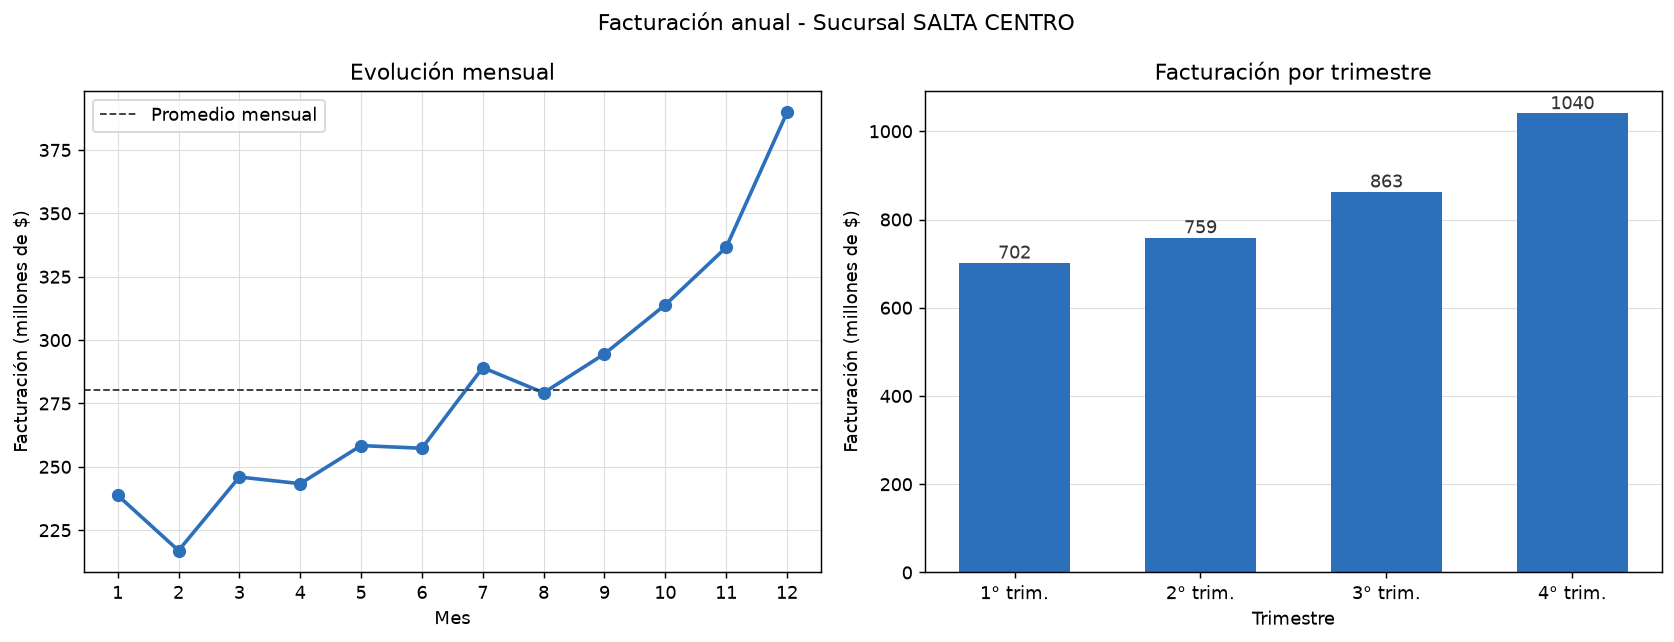
\includegraphics[width=\textwidth]{./assets/grafico_facturacion.png}
\end{center}

\subsection{Gráficos de merma (opción 8)}

La segunda figura compara la merma de cada sector contra su meta y, por separado, la pérdida expresada en dinero. Las barras son horizontales para que los nombres de los sectores se lean sin rotar, y cada meta se marca con un trazo vertical sobre su propia barra: la barra que pasa su marca es la que se desvió.

El color indica el estado, pero nunca por sí solo: junto a cada barra se escriben el porcentaje y el estado en palabras, de manera que el gráfico siga siendo legible impreso en blanco y negro o para quien no distinga el rojo del verde.

\begin{center}
    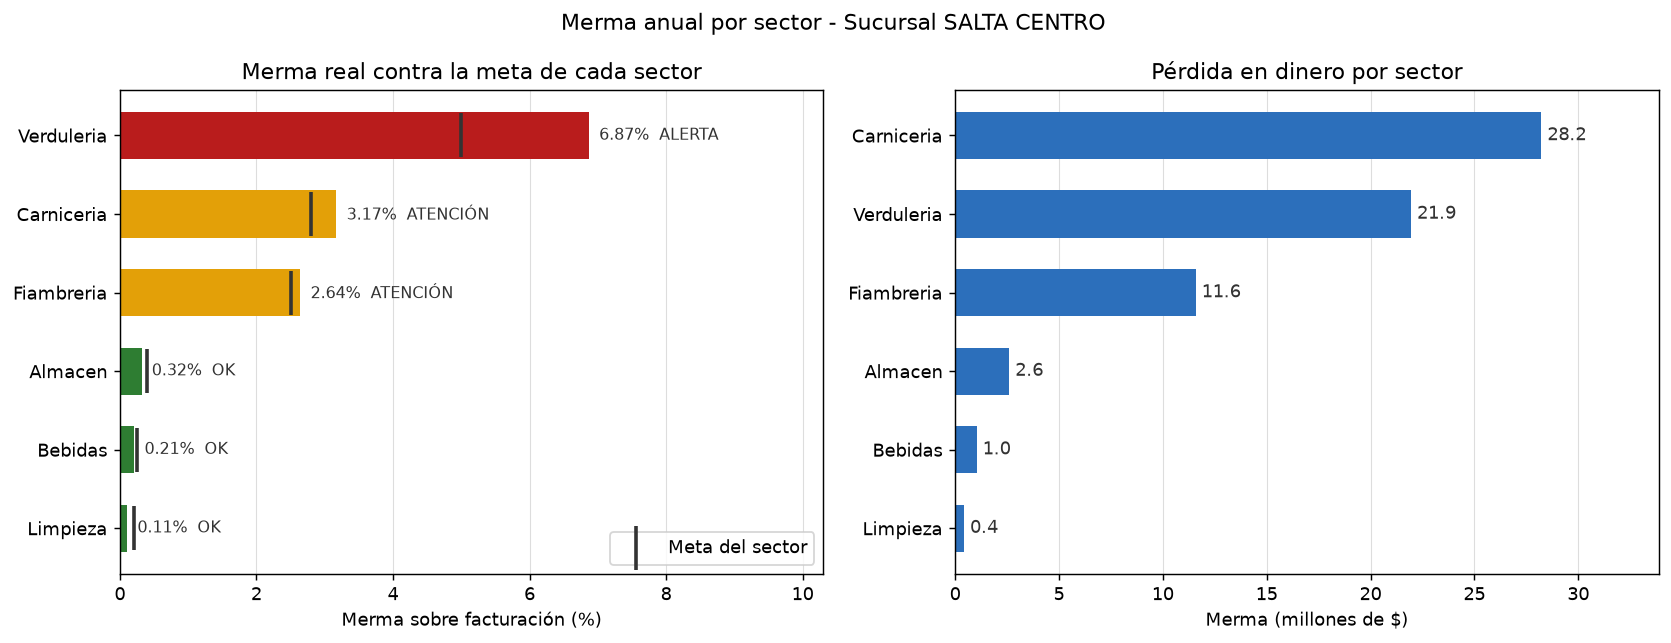
\includegraphics[width=\textwidth]{./assets/grafico_merma.png}
\end{center}

Los dos paneles están en unidades distintas (porcentaje uno, pesos el otro) y por eso se presentan como gráficos separados y no superpuestos en un mismo par de ejes. La comparación entre ambos es justamente el punto: la carnicería es la que más dinero pierde en términos absolutos, pero la verdulería, que pierde menos plata, es la que está peor respecto de lo que se espera de ella.

\volverindice

\newpage

% ============================================================
\section{Código fuente}
% ============================================================

A continuación se transcribe el contenido completo de \codigo{Examen\_Final.py}.

\lstinputlisting[style=python, caption={Examen\_Final.py}]{Examen_Final.py}

\volverindice

\newpage

% ============================================================
\section{Archivos de datos}
% ============================================================

\subsection{sectores.csv}

Archivo nuevo respecto del TP 4. Las metas se fijaron según el riesgo de cada rubro: los sectores de mercadería no perecedera admiten menos de medio punto de merma, mientras que la verdulería, que trabaja con productos que se descartan en pocos días, admite hasta cinco puntos.

\lstinputlisting[style=salida, caption={sectores.csv}]{sectores.csv}

\subsection{ventas.csv}

Es el mismo archivo del Ejercicio 14 del TP 4, con 72 registros. Se transcriben las primeras filas a modo de muestra.

\begin{lstlisting}[style=salida]
mes,sector,unidades,precio_unitario,unidades_merma
1,Almacen,48600,1200,197
1,Bebidas,19440,1800,52
1,Carniceria,9720,6500,394
1,Fiambreria,6480,4800,219
1,Verduleria,16200,1400,1422
1,Limpieza,12960,2200,17
2,Almacen,42300,1250,165
...
\end{lstlisting}

\volverindice

\end{document}
